
\section{Existing ontology work}
\label{existingontologies}

One of the key aspects of FAIR ontologies is that they are reusable and profit
from the reusability of existing ontologies \cite{PovedaVillalon.2020}. We did
an extensive analysis of existing ontologies with infrastructure, charging
stations, electric vehicles and electricity grid in scope. We also rely
strongly on the review performed by Katsumi and Fox regarding transport
planning vocabularies \cite{Katsumi.2018}. In this section we summarize the
ontologies we considered for reutilization and justify the situations in which
we decide not to reutilize existing concepts.


\subsection{The Open Energy Ontology}

The OEO has been in active development since 2021 with several releases since
then. It exists to address a technical gap associated with knowledge management
in the field of energy systems analysis. Said gap is the lack of common
semantics to annotate and share datasets and tools associated with the
mentioned discipline. The ontology is part of a larger data ecosystem called
the Open Energy Family (OEF), which allows researchers to share data sources
and results in accordance with the FAIR principles. It has had moderate
success, particularly within the context of projects associated to the OEF such
as the Open Energy Platform (OEP) \cite{Hulk.2024}. One of the characteristics
that makes this and other FAIR ontologies transparent and accessible is the
fact that it is being openly developed in a shared
repository\footnote{https://github.com/OpenEnergyPlatform/ontology}. An
important work on the inclusion of concepts coming from the transport sector
was performed by \cite{Mittermeier.2023}, who did several implementations
associated to the topic. However since the size of the task is larger than what
can be achieved during a master thesis, many implementations were left open in
the form of GitHub Issues. In some of these issues it was made clear that the
scope of the OEO is in some cases beyond what is often necessary to represent
phenomena in the transport sector.


In our charging infrastructure ontology we need a way of describing vehicles,
particularly electric vehicles. The OEO has a rich taxonomy of vehicles that
rest on the definition of artificial objects which are in the context of BFO
`causally unified material entities deliberately manufactured by humans to
address a particular porpoise'. The taxonomy has multiple parallel
ramifications, one associated to its energy consumption mode like `electric
vehicle', `internal combustion vehicle' and `gas turbine vehicle' and another
associated to its operational medium such as `land vehicle', `aircraft' or
`watercraft'. The former has axiomatization significant for electric grid and
energy systems models which can be seen in figure \ref{oeoev:b} the latter
lacks its own axioms and relies on mainly on the former. For our application is
only interesting to use the taxonomy of electric vehicles (Figure
\ref{oeoev:a}). Its land vehicle taxonomy is very rich (figure
\ref{landvehicletaxoeo}) and contains elements that might have conflicts with
any future implementation in a transport ontology. Because of this we rely on
the Common Core Ontologies (CCO) for a ligther vehicle taxonomy, this will be
clarified in its respective section.

\begin{figure}
    \centering
    \subfigure[OEO electric vehicle taxonomy]{\label{oeoev:a}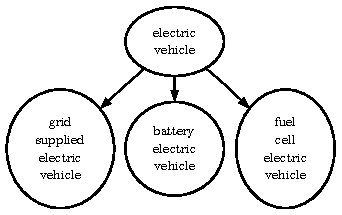
\includegraphics[width=0.45\textwidth]{images/OEOVehicles}}
    \subfigure[OEO electric vehicle commitments]{\label{oeoev:b}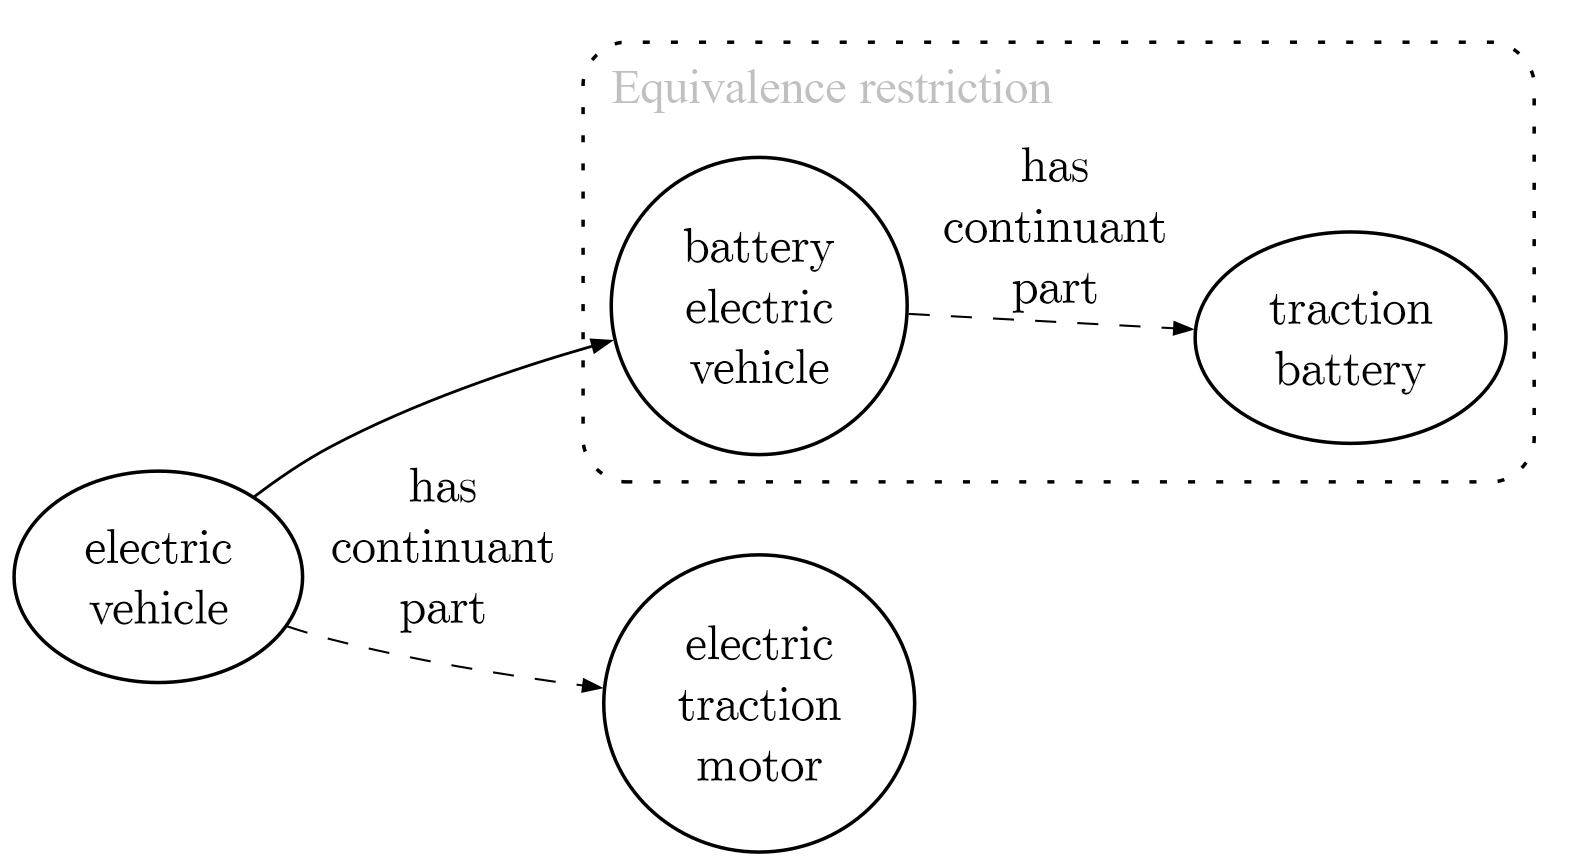
\includegraphics[width=0.45\textwidth]{images/OEOEV}}
    \caption{OEO ontological commitments relevant to the context of charging infrastructure. Note that we exclude grid related commitments, mostly because we have yet to define a scenario for that case.}
\end{figure}

\subsection{The Common Core Ontologies}

The CCO are 12 mid-level ontologies built as an extension of BFO and the
Relations Ontology (RO) intended to be used as a basis to model domains of
interest such as transportation infrastructure spacecrafts
\cite{Rudnicki.23September2020}. Like BFO, it is a realist ontology, which
means that it intends to model entities and data alike. The ontology avoids
being prescriptive, instead lets data modellers decide which asserted class
axioms are relevant for their particular applications. The ontology comes with
a guide that lets non ontology experts understand how to implement terms in the
ontology which is very helpful to involve domain experts of other fields in
ontology development.

We import a small subset of terms coming from these ontologies. Indeed, we
avoid importing whole ontologies by opting to do punctual extractions. This was
decided to avoid convolution of the final product, since we are expecting
developers to work with Protégé, if we imported all the classes they would have
a harder time finding where to place their new terms. We extract multiple
taxonomies and some axioms from these ontologies. These are listed during the
rest of this section.

\subsubsection{Vehicle taxonomy}

From the artifact ontology we extract terminology associated with vehicles. We
consider that their non-prescriptive approach offers a more manageable taxonomy
of vehicles that can be utilized across different fields of application. The
OEO classifies vehicles based on their energy consumption which is practical
for their applications but since we are not interested in non-electric vehicles
these become superfluous. Other reason to use the artifacts ontology
axiomatization is to profit from the other declarations coming from the same
suite of ontologies, particularly the axioms that allow `material artifacts'
with `sites' which will be helpful to handle concepts associated with parking.
The top upper levels of both taxonomies, besides both using BFO are slightly
different. The OEO classifies vehicles as artificial objects whereas the CCO as
`material artifacts'. The lower levels, despite being developed independently
are very similar, so similar  that they are practically already interoperable.
The taxonomies can be compared by looking at figures \ref{ccovectax} and
\ref{landvehicletaxoeo}.

\begin{figure}[h]
    \centering
    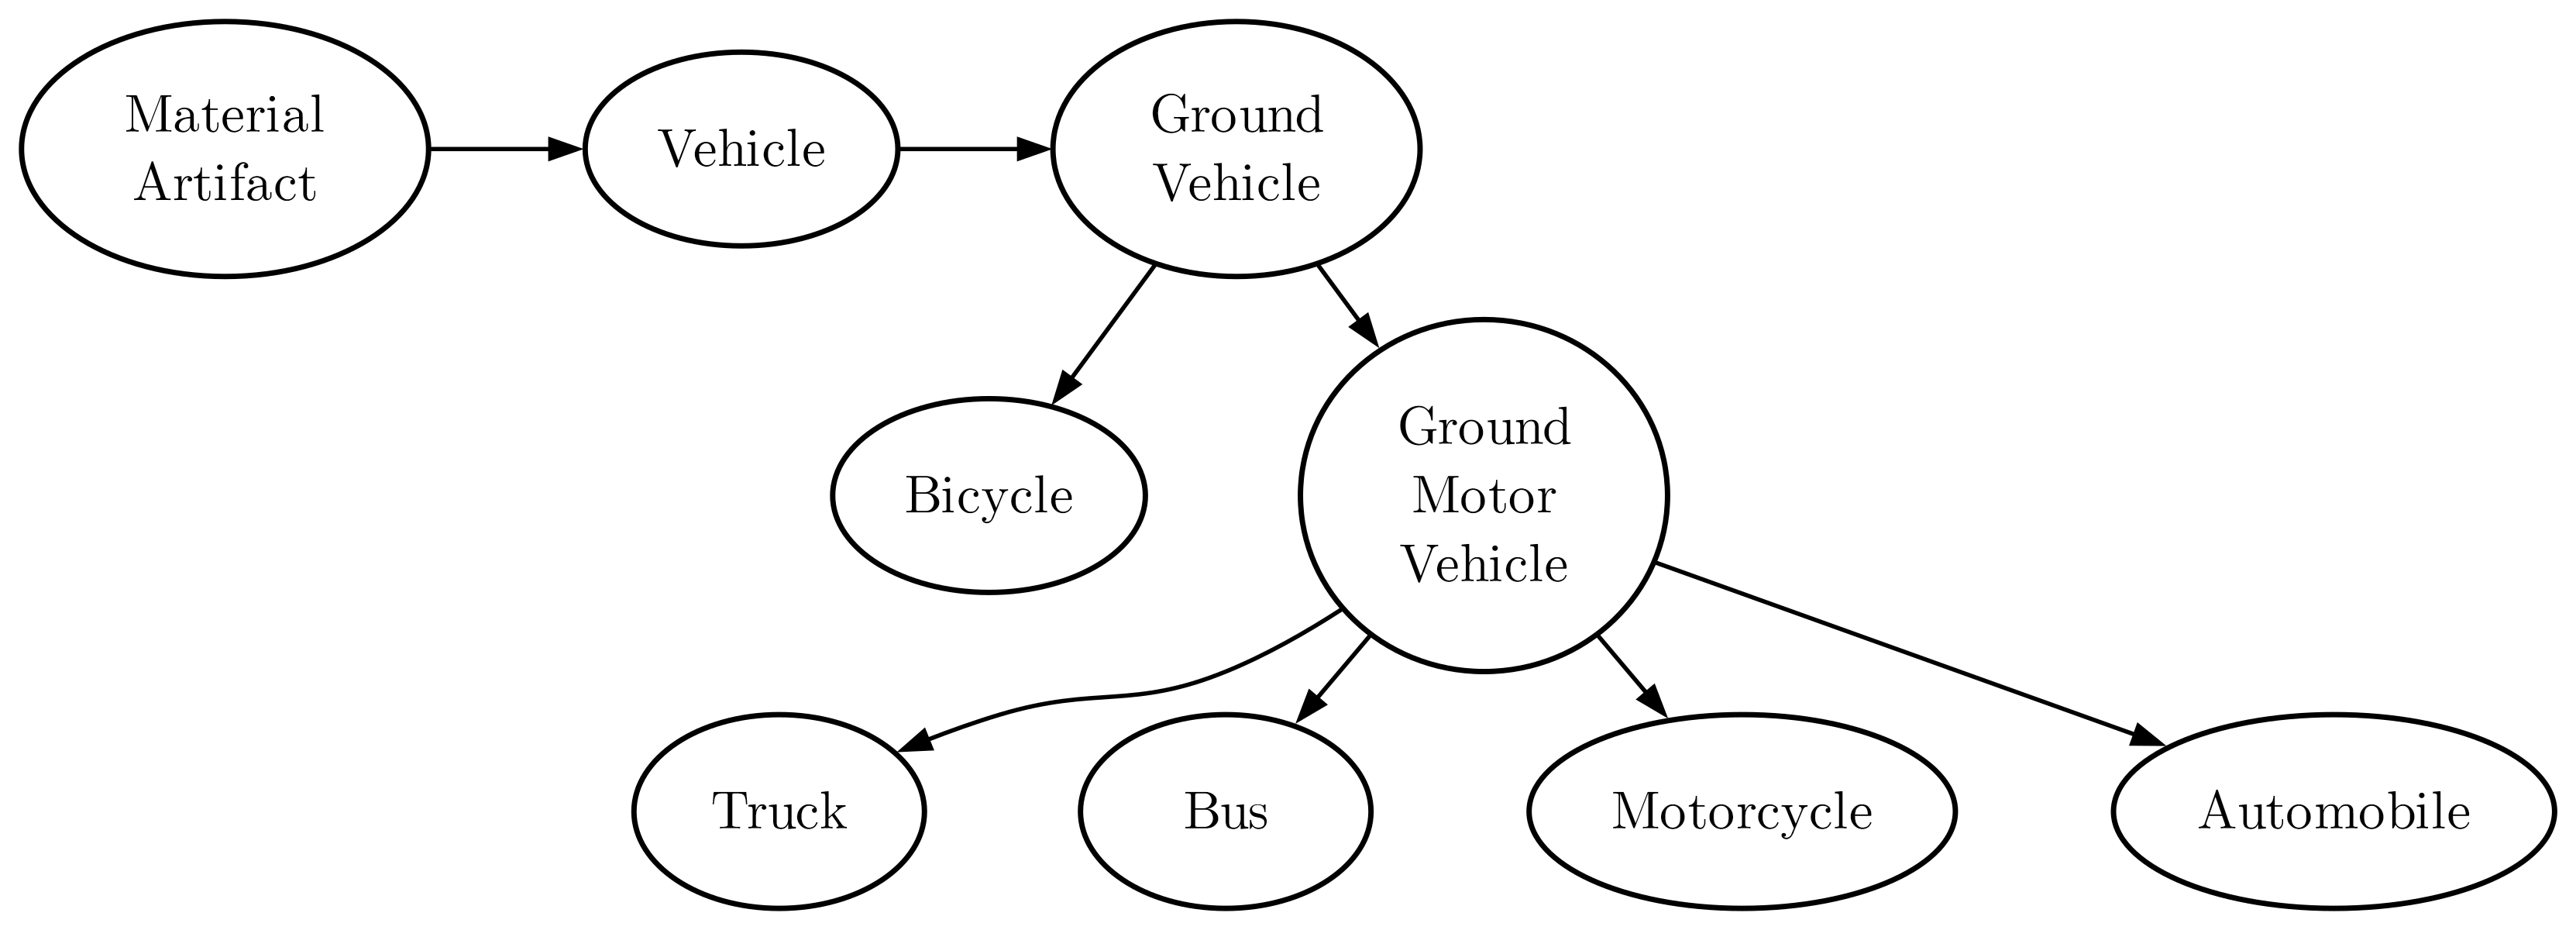
\includegraphics[width=0.9\textwidth]{images/CCOVehicles}
    \caption{The CCO vehicle taxonomy is slimmer and more streamlined to the concept of a vehicle.}
    \label{ccovectax}
\end{figure}
\begin{figure}[h]
    
    \centering
    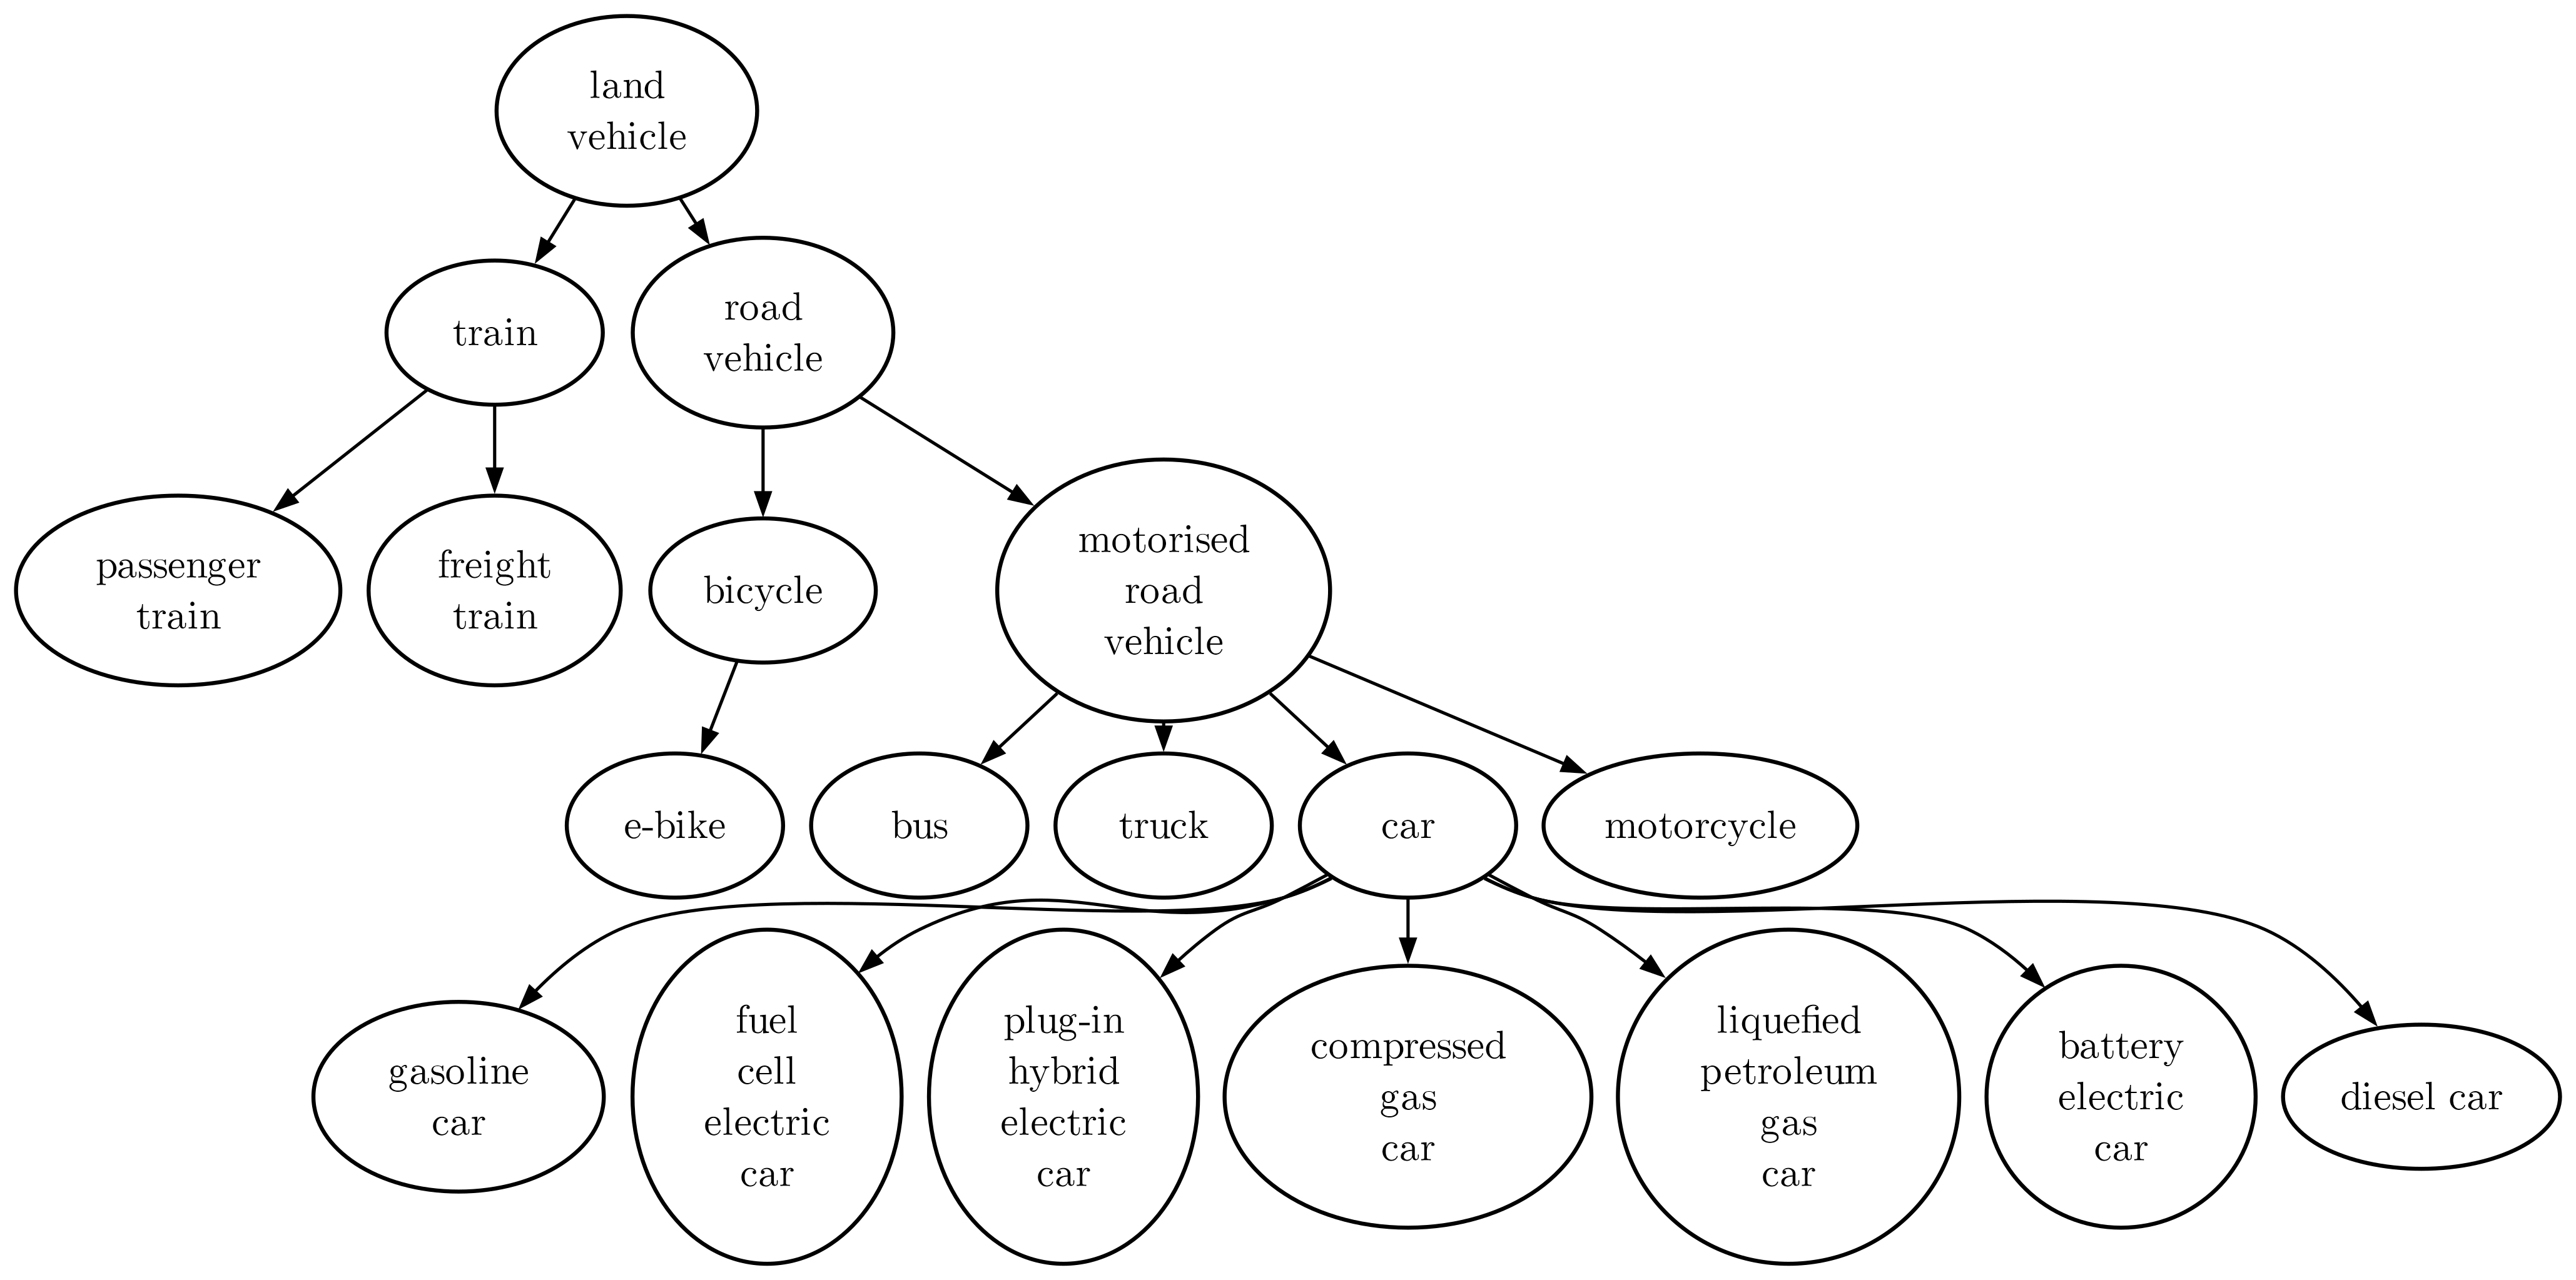
\includegraphics[width=0.9\textwidth]{images/OEOLVehicles}
    \caption{The OEO Land vehicle taxonomy is rich of axioms associated to the vehicles' energy consumption.}
    \label{landvehicletaxoeo}
\end{figure}

\subsubsection{Infrastructure}

The CCO offers a construct that aids to classify material artifacts as
infrastructure. It uses what in BFO are called `roles'. This allows arbitrary
assignment of the class. This is practical to us because charging stations in
reality are not always infrastructure, they are only in virtue of the agents
who assign them this role. In this sense a home wall box is not infrastructure
for a government agency but a public column is. Infrastructure rarely comes as
units but as  complex aggregates of artifacts, this is way we opt to import the
concept of infrastructure system. These axioms can be visualized in figure
\ref{infrastructurefigs}.

\begin{figure}[h]
    \centering
    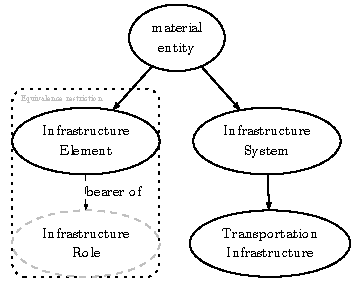
\includegraphics[width=0.8\textwidth]{images/infrastructureSystem}
    \caption{Common Core Ontologies infrastructure constraints.}
    \label{infrastructurefigs} 
\end{figure}

\subsubsection{Facilities}

As an only exception to our `scenario first' rule we import the facility
ontology to handle concepts like parking lots and dedicated charging stations.
An alternative would be to stick to using material entities, but we consider
this differentiation practical in the long run. Specially when considering
interoperability with future transportation research ontologies


\subsection{iCity Parking ontology}

The TPSO has a module for terminology associated with parking which provides
concepts like parking spaces, areas and fees. It also offers definitions for
charging stations, but these are too shallow for our applications as they are
at most features of parking spaces. The subclassification of charging stations
are `standard', `medium' and `fast' which are defined based on the definitions
of the Environmental Protection Department whose source was not explicitly
pointed. If having such a classification is meaningful to our applications is
yet to be defined. The TPSO has its own upper level ontology modules which
supply axiom definitions for change, mereology and time. These modules are
fundamentally incompatible with the BFO. The Change module of the ontology
relies on the utilization of a 4 dimensional approach to model time changing
concepts. This means that every object has a perdurant and its manifestations
bear their changes. Since we are not intending to axiomatize time relations in
OWL and instead opt to delegate that to data modellers we opt not to share that
approach. All the axioms that are interesting to us from the Parking ontology
can be visualized in figure \ref{parkingfig}. BFO has its own approach to
handle descriptions of change, this will be addressed in its respective
section.

\begin{figure}[h]
    \centering
    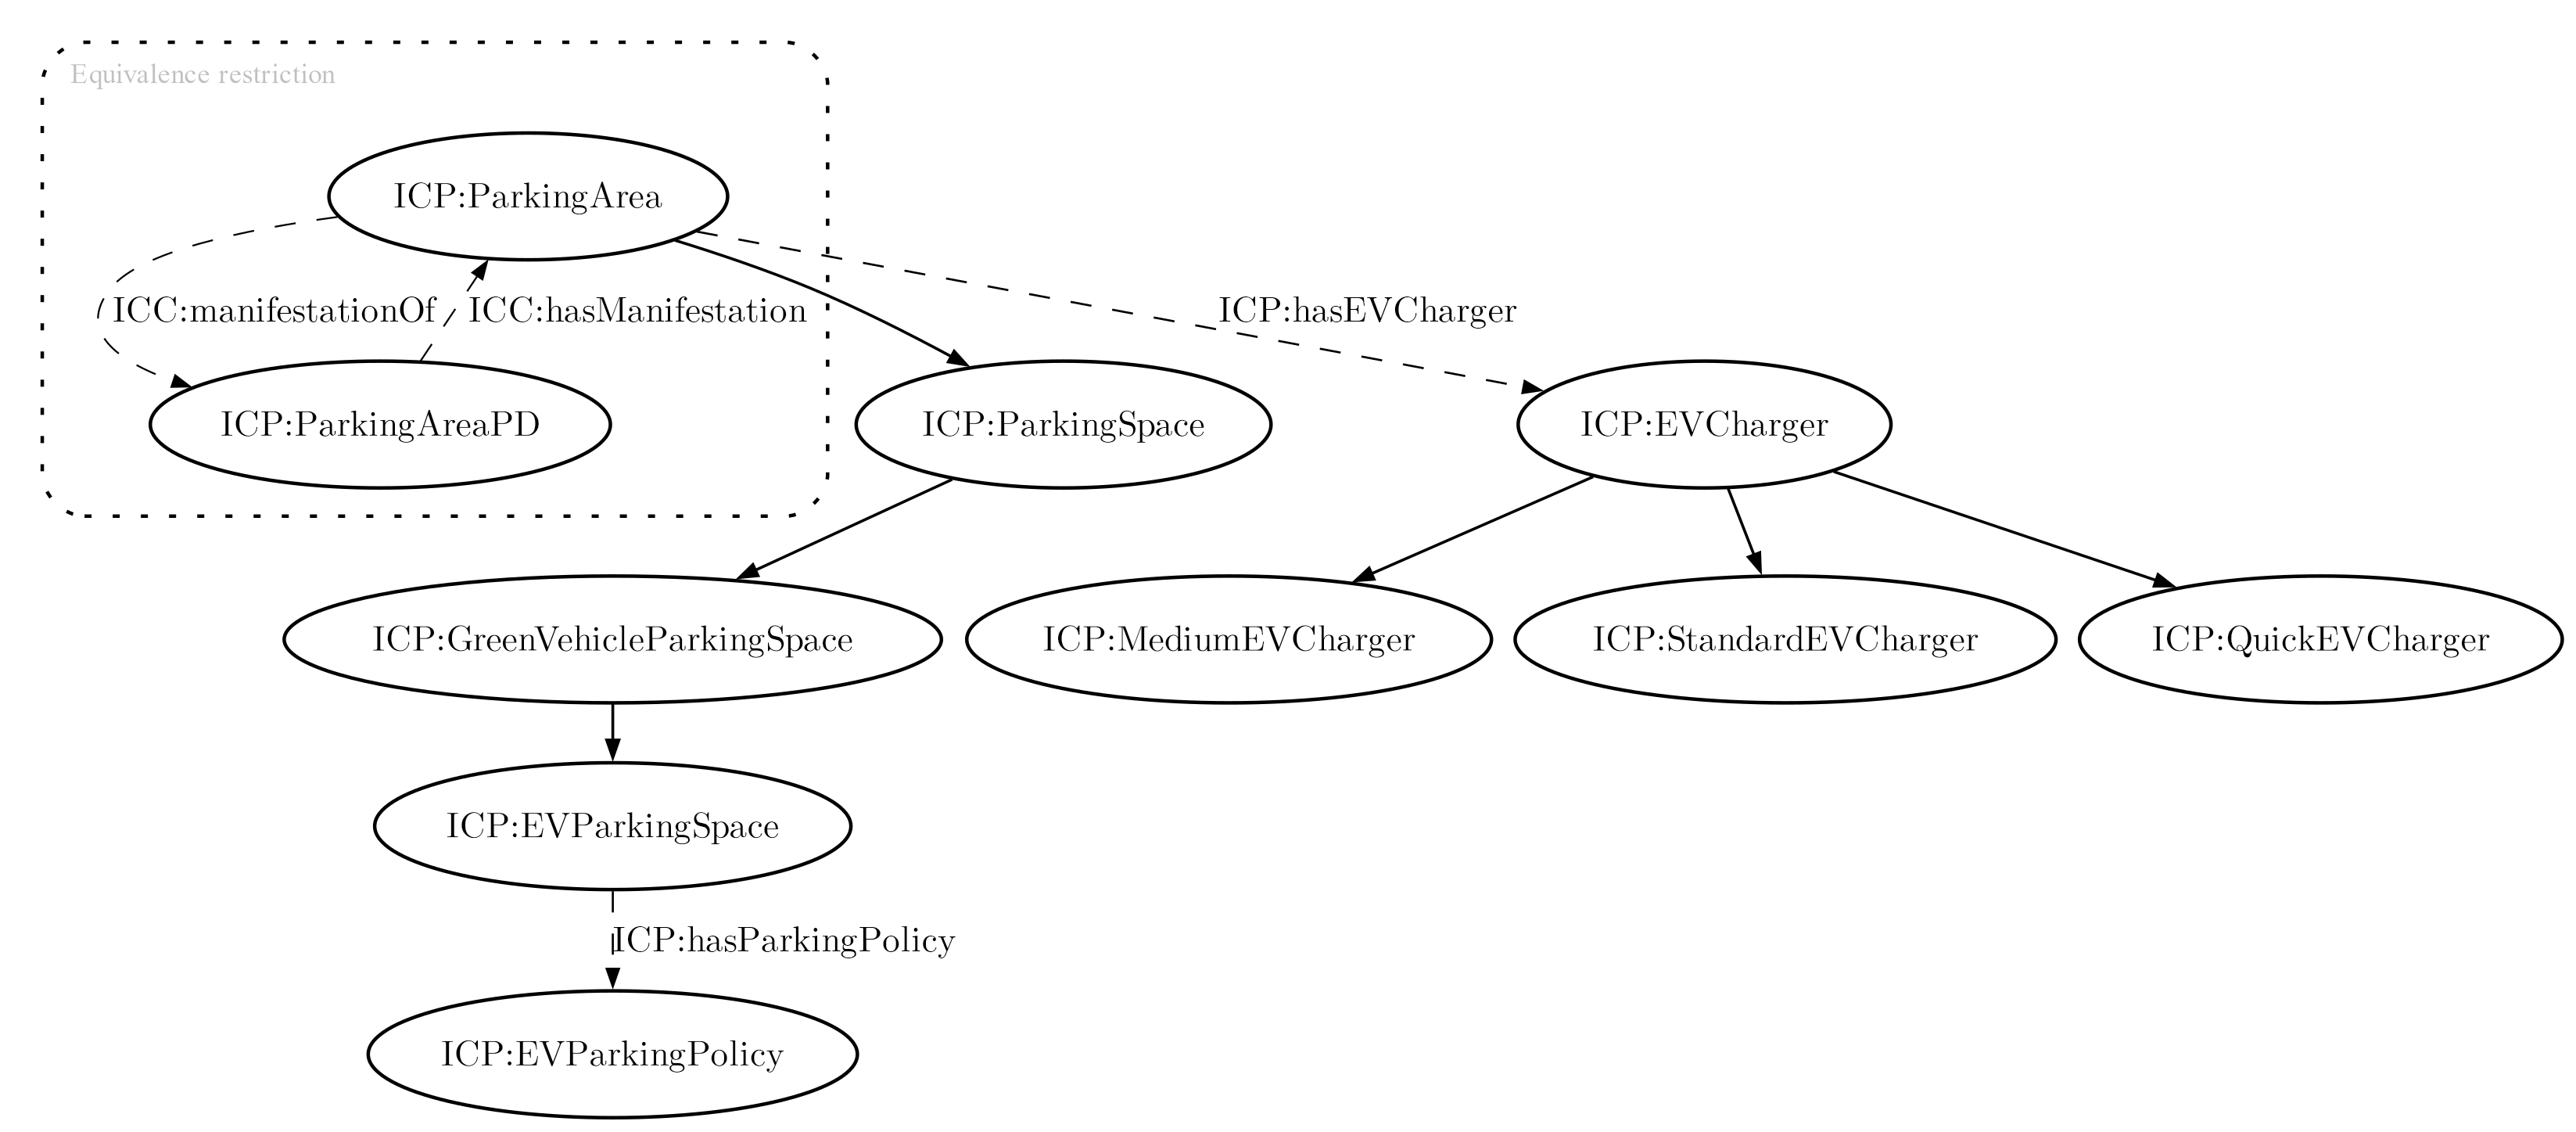
\includegraphics[width=1.0\textwidth]{images/PARKING}
    \caption{iCity parking ontology commitments associated to charging infrastructure.}
    \label{parkingfig}
\end{figure}

\subsubsection{The Basic Formal Ontology}
\label{upperlevel}

Top-level ontologies or foundational ontologies intend to model domain neutral
categories and relations \cite{Arp.2015}. These are not a hard requirement to
build an ontology but can make the difference regarding its interoperability.
Choosing (or developing) a top-level ontology is not an easy task because a
modeller needs to have a deep understanding of their domain and the possible
applications. In 2022 a special issue of applied ontology \cite{Borgo.2022}
allowed ontology developers to exemplify the usage of multiple prominent
top-level ontologies. In theory, we would select our ontology by following the
motivating scenarios defined in section \ref{methodology}. But since we are
intending to build on the efforts from the OEO we streamlined to using BFO.
This decision comes not without compromises. 

BFO sacrifices expressivity for a simpler modelling intuition. It has
weaknesses in the field of modal propositions which are prominent in both
transportation research en energy systems analysis, particularly in the context
of forecasts and simulation\footnote{However this weakness is addressed by CCO
with their ModalRelationOntology which we consider importing. }. Unlike the
TPSO foundational modules, BFO delegates its time indexing to the applications
by keeping it outside the OWL implementation. BFO has a rather simple initial
learning curve that can be used to facilitate the inclusion of new developers.
But still becomes very steep when dealing some of its more complex terms (i.e.
`process profile', `disposition' vs `quality'), this can lead to frustrations
or miss-uses.

There are some important features of BFO that we intend to take advantage of.
The first is that it allows the existence of `sites' in the same dimension as
`material entities'. This is because charging events depend on the dynamics of
vehicles being present and absent. We also need these entities to characterize
the mereotopology of charging stations which usually consider parking spaces as
their parts. A second important feature are `process profiles', since we
consider that the charging event can have multiple dimensions that can describe
it that have to be associated with each other. Using those we can describe
events in virtue of their occupancy, power rates and energy transfers.
